\documentclass[letterpaper,12pt]{article}
\usepackage[utf8]{inputenc}
\usepackage{charter}
\usepackage{geometry}
\usepackage{amsmath}
\usepackage{float}
\usepackage{graphicx}
\usepackage{subcaption}
\usepackage{amssymb}
\usepackage{adjustbox}
\usepackage{wrapfig} 
\usepackage{xcolor}
\usepackage{fancyhdr}
\usepackage{tabularx}
\usepackage{fancyhdr}
\usepackage{comment}

\geometry{top=2cm, bottom=2cm, left=2cm, right= 2cm} %%margen
\graphicspath{{images/}}
\parindent=0pt

\begin{document}
%%para contador y eso
\thispagestyle{empty}
\newpage
\setcounter{page}{1}
\pagestyle{headings}
%%%%%%%%%%%%%%%%%%%%%%%%%%%%%%%%%%%%%%%%%%%%%%%%%%%%%%%%%%%%%%%%%%%%%%%%%%%%
\begin{sloppypar} 
    %%%portadita
\begin{titlepage}
    \fancyhead{R}{
    
\includegraphics[width=0.1\linewidth]{logoUV.png}
    }
    \hspace{2.5cm}
    {\bfseries\LARGE Universidad Veracruzana \par}
    \hspace{2cm}
    {\scshape\Large Facultad de Ingeniería Eléctrica y Electrónica \par}
    \begin{center}
        \vfill
        {\Huge \textbf{B-TREE}} \\ 
        {\itshape\Large Estructura de Datos \par}
        {\large Lara Xocuis Martha Denisse \par}
        {\large S22002213 \par}
        \vfill
        {\Large \today \par}
    \end{center}
    
\end{titlepage} 

%%%%%%%%%%%%%%%%%%%%%%TOPOLOGÍA%%%%%%%%%%%%%%%%%%%%%%
\section{Características y propiedades de un árbol B}
\begin{figure}[H]
    \centering
    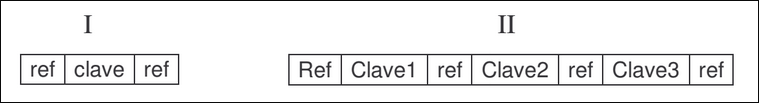
\includegraphics[width=0.8\textwidth]{b.png}
\end{figure}
k : Cantidad máxima de claves por nodo \\ 
m : Cantidad máxima de hijos por nodo \\ 
\vspace{0.3cm}\\ 
Si conocemos el número máximo de claves (k), se puede calcular:




\end{sloppypar}
\end{document}